\section{Technical overview}

\subsection{DonkeySimulator}

When it comes to simulators, we had 2 options: 
\begin{enumerate}
\item Udacity Simulator
\item DonkeySimulator
\end{enumerate}

\begin{figure}[!h]
\centering
\begin{minipage}[t]{6cm}
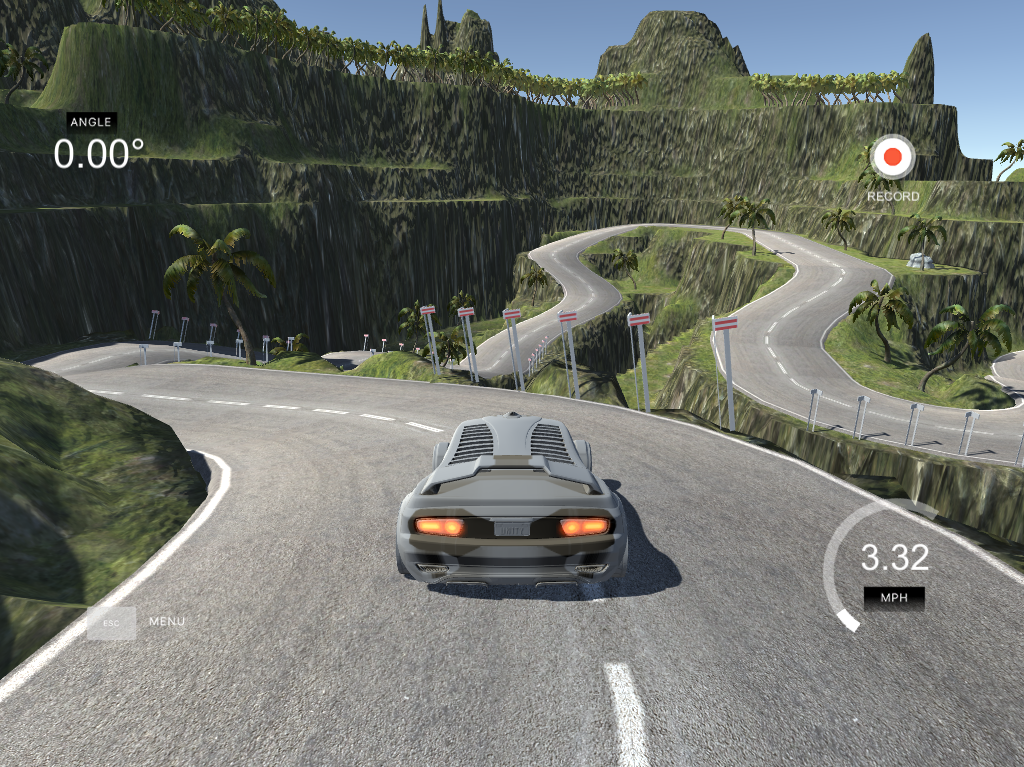
\includegraphics[width=6cm]{img/udacity_sim.png}
\caption{Udacity Simulator}
\end{minipage}
\hspace{1cm}
\begin{minipage}[t]{8cm}
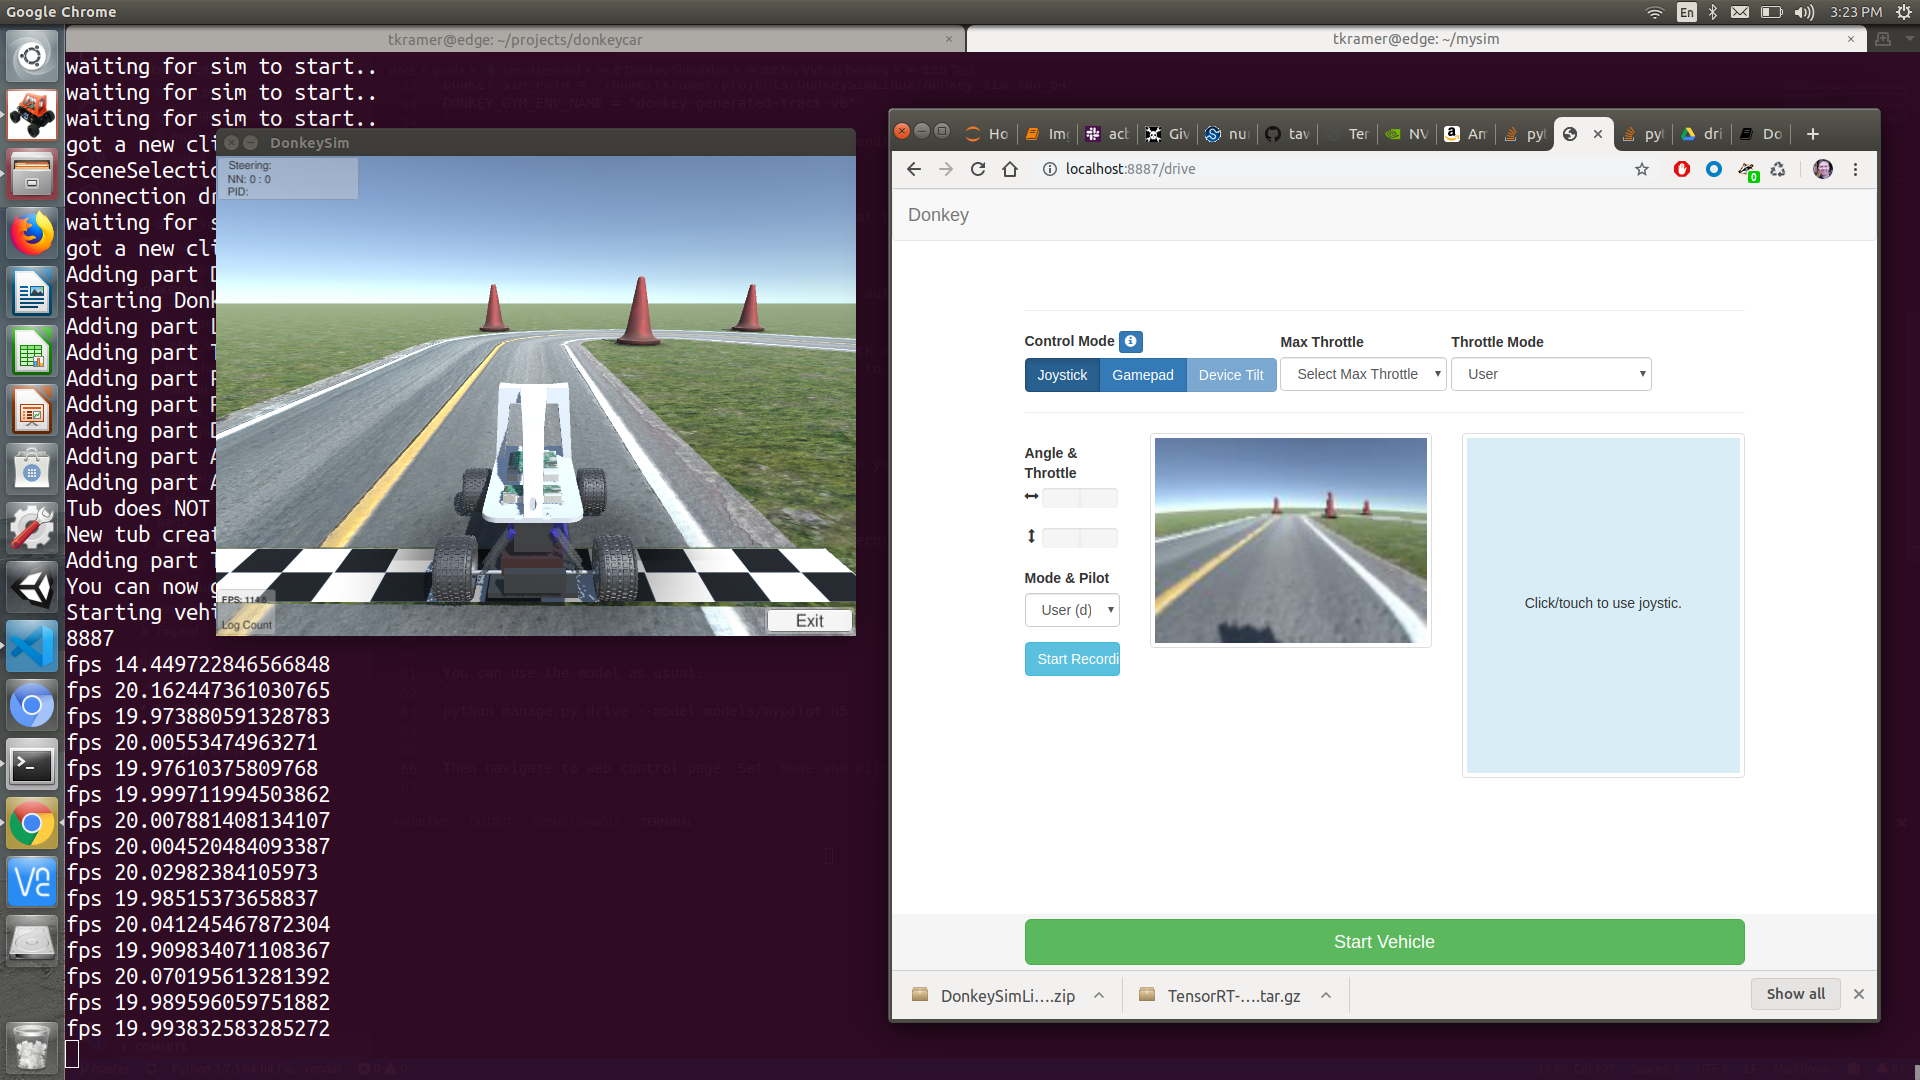
\includegraphics[width=8cm]{img/donkey_sim.png}
\caption{DonkeySimulator}
\end{minipage}
\end{figure}

We decided not to choose the udacity simulator, even though closest to the reality than the DonkeySimulator. ``Why ?'', you may ask. It's because the DonkeySimulator has a built-in track really similar to the one where our car is going to drive the D-day. Moreover, it's easy to implement a second camera to the car, or even simulate the compute power of a \makebox{\textbf{Raspberry pi}}. There's even an OpenAi-Gym environnment !


\begin{figure}[!h]
\centering
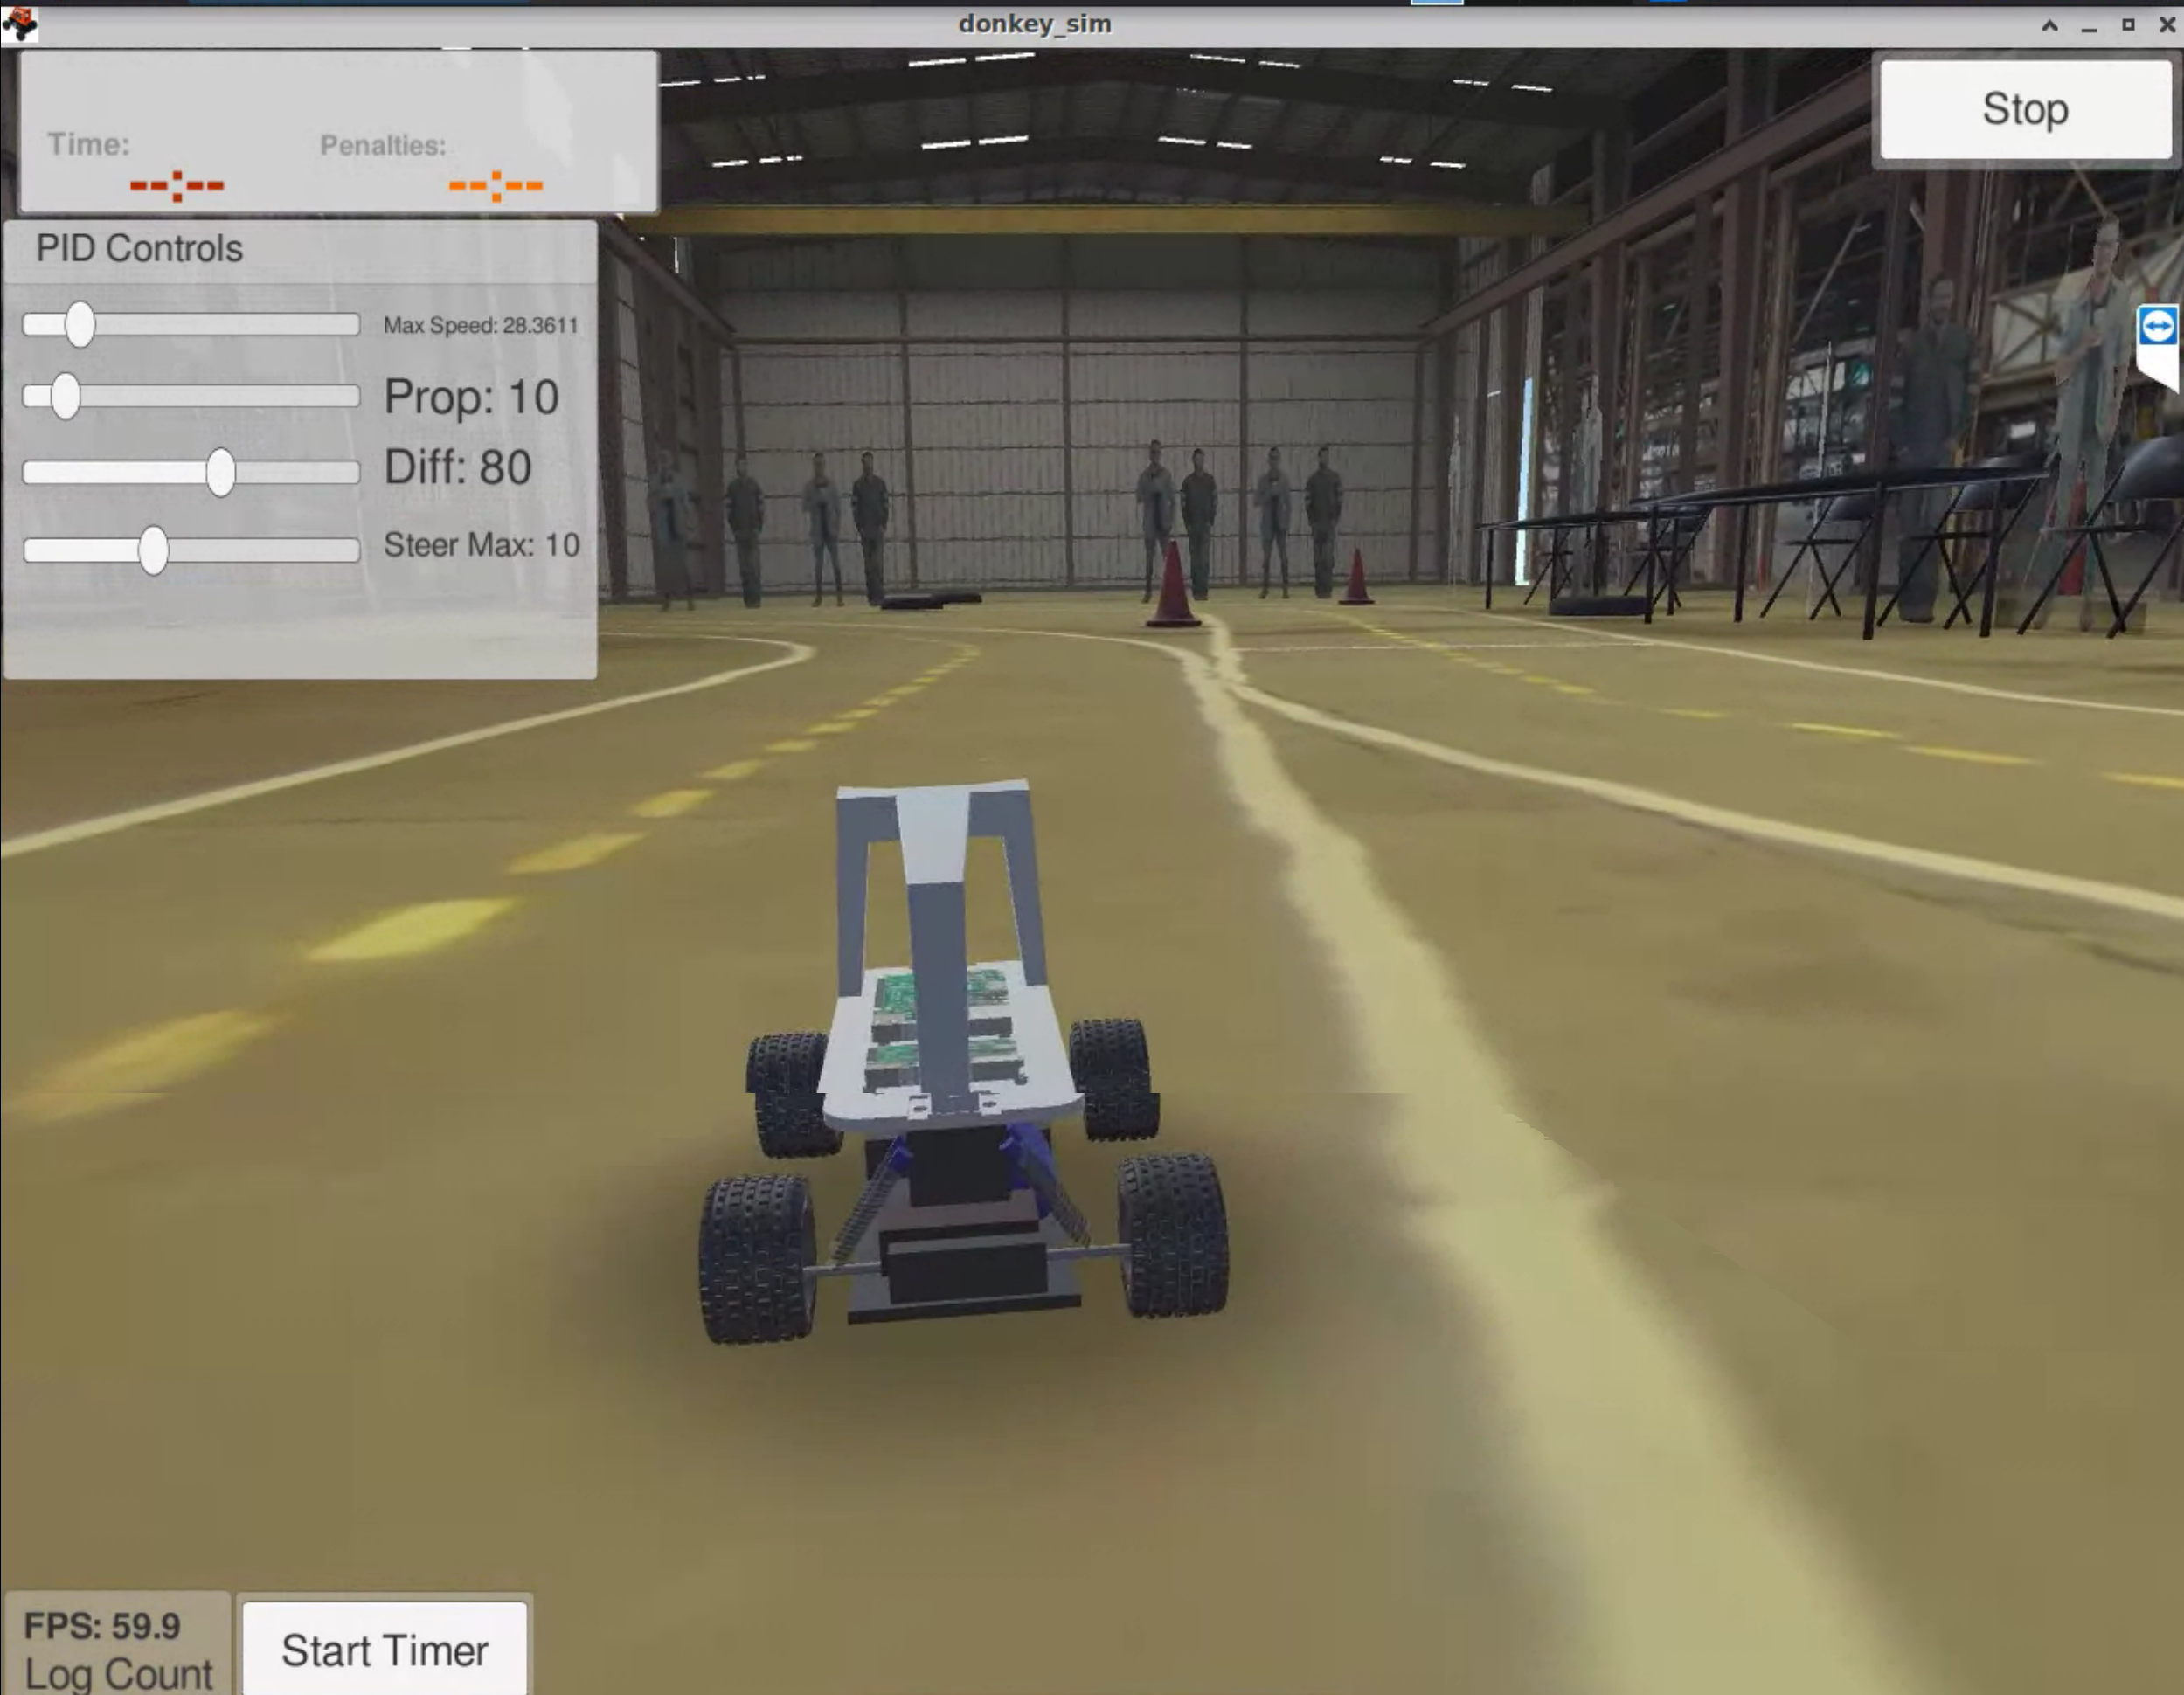
\includegraphics[width=10cm]{img/track.png}
\caption{The track on DonkeySim is really similar to the real one}
\end{figure}
\clearpage

\subsection{Dataset}

We started the project mid-november and we still, at this day, do not have a physic car. In the other hand, we needed to start training models to choose the most efficient. Our only option was to find online dataset to start training a model, and then, when we'll receive the car, we'll just have to transfer it in the car.\\





\subsection{Our model choice}

First we need to plant the basics. What our AI model needs to make predictions on ? Our model will make live predictions on the steering and the throttle of our car using images given by the camera on the car.\\

What is the best algorithm ? Which one is the most relaible, efficient ?\\

We have several options and this part, we will present the pros and the cons of the algorithm selection that we have made.\\

We will be using the Keras (open-source sofware library with a python interface) high level API in combination with a Tensorflow backend.\\ 

\subsubsection*{Keras Categotical}

\begin{table}[!h]
\begin{center}
\begin{tabular}{|p{6cm}|p{6cm}|}
\hline
\textbf{Pros} & \textbf{Cons}\\
\hline
It has some benefits of showing the confidense as a distribution via the makemovie command & Suffers from some arbitrary limitations of the chosen limits for number of categories, and thottle upper limit \\
\hline
It has been very robust & \\
\hline
In some cases this model has learned thottle control better than other models & \\
\hline
Performs well in a limited compute environment like the Pi3 & \\
\hline
\end{tabular}
\end{center}
\caption{Keras Categorical Pros/Cons}
\end{table}



\subsubsection*{Keras Linear}

\begin{table}[!h]
\begin{center}
\begin{tabular}{|p{6cm}|p{6cm}|}
\hline
\textbf{Pros} & \textbf{Cons}\\
\hline
Steers smoothly & May sometimes fail to learn throttle well \\
\hline
It has been very robust & \\
\hline
No arbitrary limits to steering or throttle  & \\
\hline
Performs well in a limited compute environment like the Pi3 & \\
\hline
\end{tabular}
\end{center}
\caption{Keras Linear Pros/Cons}
\end{table}

\subsubsection*{Keras IMU}

\begin{table}[H]
\begin{center}
\begin{tabular}{|p{6cm}|p{6cm}|}
\hline
\textbf{Pros} & \textbf{Cons}\\
\hline
Steers very smoothly  & Driving quality will suffer if noisy imu is used \\
\hline
Performs well in a limited compute environment like the Pi3  & \\
\hline
No arbitrary limits to steering or throttle  & \\
\hline
Gives additional state to the model, which might help it come to a stop at a stop sign & \\
\hline
\end{tabular}
\end{center}
\caption{Keras IMU Pros/Cons}
\end{table}


\subsubsection*{Keras Latent}

\begin{table}[H]
\begin{center}
\begin{tabular}{|p{6cm}|p{6cm}|}
\hline
\textbf{Pros} & \textbf{Cons}\\
\hline
Steers smoothly  & Needs more testing to prove theory  \\
\hline
Performs well in a limited compute environment like the Pi3  & \\
\hline
No arbitrary limits to steering or throttle.  & \\
\hline
Image output a measure of what the model has deemed important in the scene & \\
\hline
\end{tabular}
\end{center}
\caption{Keras Latent Pros/Cons}
\end{table}

\subsubsection*{Keras RNN}

\begin{table}[H]
\begin{center}
\begin{tabular}{|p{6cm}|p{6cm}|}
\hline
\textbf{Pros} & \textbf{Cons}\\
\hline
Steers very smoothly  & Performs worse in a limited compute environment like the Pi3\\
\hline
Can train to a lower loss   & Takes longer to train \\
\hline
\end{tabular}
\end{center}
\caption{Keras RNN Pros/Cons}
\end{table}


\subsubsection*{Keras Behaviour}

\begin{table}[H]
\begin{center}
\begin{tabular}{|p{6cm}|p{6cm}|}
\hline
\textbf{Pros} & \textbf{Cons}\\
\hline
Can create a model which can perform multiple tasks & Takes more effort to train \\
\hline
\end{tabular}
\end{center}
\caption{Keras Behaviour Pros/Cons}
\end{table}

\subsubsection*{Keras Localizer}

\begin{table}[H]
\begin{center}
\begin{tabular}{|p{6cm}|p{6cm}|}
\hline
\textbf{Pros} & \textbf{Cons}\\
\hline
Steers smoothly  & May sometimes fail to learn throttle well  \\
\hline
Performs well in a limited compute environment like the Pi3  & \\
\hline
No arbitrary limits to steering or throttle.  & \\
\hline
Location to supply some higher level logic & \\
\hline
\end{tabular}
\end{center}
\caption{Keras Localizer Pros/Cons}
\end{table}


\subsection{Lane Detection algorithm}

The first to do was to create a simple lane detection algorithm, by assuming that all line will be straight. We used \textbf{OpenCV}, an open-source computer vision library, usable both in Python and C++. This tool include image processing, camera calibration, object detection\dots \\

\begin{figure}[!h]
\centering
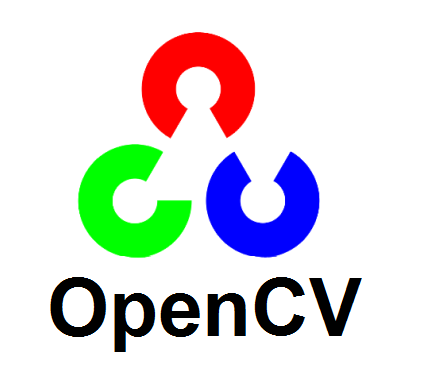
\includegraphics[scale=0.25]{img/opencv.png}
\caption{OpenCV is an Open-source Computer Vision Library}
\end{figure}

The usual methodology in this case is as follow:\footnote{Cf. appendix \ref{laneDetect} for the complete code and appendix \ref{imagelaneDetect} for the pictures}
\begin{enumerate}
\item Put image in gray in order to emphasize the white lines
\item Blur the immage using a \textbf{Gaussian Filter}\footnote{By averaging the values of nearby pixels, the Gaussian Filter reduce the noise in the image}
\item Use the \textbf{Canny} algorithm to find edges on the image
\item Cropp the image only where the lines should be
\item Using the \textbf{Hough} algorithm to find lines in the resulted image
\item Select the average left line and right line from the array of lines
\item Finaly display the line on top of the image (or frame in case of a video)
\end{enumerate}



\clearpage
\subsection{OpenAI Gym}

\begin{figure}[!h]
    \centering
    \def\svgwidth{0.7\columnwidth}
    \input{openai.pdf_tex}
\end{figure}

OpenAI, one of the most famous company in the Deep Learning domain, has developped an open-source framework to help the implementation of a certain type of deep learning algorithm. This kind of algorithm is particularly efficient when it comes to\dots~playing games !\\

In fact, OpenAi-Gym is best suited for \textbf{Reinforcement Learning}, a genre of neural network were the agent is rewarded when taking good actions and penalized when doing bad things. These neural network are complicated to implement in the real world, imagine a car having to crash thousands of time before learning to turn left ! But that doesn't mean they are bad ! In fact, it's kind of the opposite: remember \textbf{AlphaGo Zero} ? It's the first algorithm to defeat the world champion of Go\footnote{Go is a game with more than $10^{17}$ possible board configuration\cite{AlphaGo}} in a 1vs1 match, and it was using reinforcment learning !\\

\subsubsection*{Reinforcement Learning}
\begin{figure}[!h]
\centering
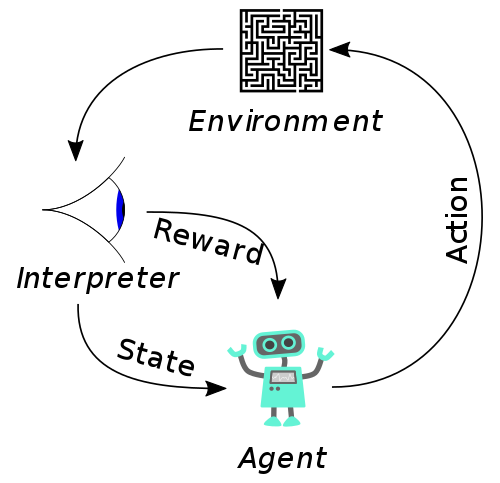
\includegraphics[width=10cm]{img/Reinforcement_learning_diagram.png}
\caption{Schematic of the reinforcement learning algorithm}
\end{figure}
\clearpage

In order to train a Reinforcement Neural Network, we have to provide it 2 differents things at each step:
\begin{itemize}
\item A state
\item A reward
\end{itemize}
And the neural network will output an action which is going to have an impact on the environment. Then the loop repeat itself.\\

In \textbf{Python}, OpenAi Gym is implemented as follow:

\subsubsection*{OpenAi Gym in Python \cite{OpenAI}}
\texttt{Steps} stipulate how long the networks is going to run (it has to be an Integer). At each step, \texttt{Observation}, \texttt{Reward}, \texttt{Done} and \texttt{Info} are outputed.\\

\texttt{Observation} represent all the data fed to the agent at a given step, it can be pixel data such as in a picture, speed, memory.\footnote{One of the goal of OpenAi Gym was to make an AI able to beat most of the NES game with only the raw memory as observation} The observation differ depending on the task, so it's taking the form of an \texttt{object}.\\

\texttt{Reward} is a \texttt{float}, positive or not, given to the agent after he took an action. The goal of the agent is to maximise the total reward.\\

\texttt{Done} is a \texttt{boolean}. When set to \texttt{True}, it indicate that the episode has terminated (either the task has failed, or the task was successfuly handled).\\

\texttt{Info} is a \texttt{dictionnary} containing information for the developper (often used for debuging). The agent is not allowed to access these informations.\\

\texttt{Space} is either a \texttt{set} or a \texttt{box}\footnote{Depending if the action space is continous or discrete} containing all the possible \texttt{Actions} that the agent can take.\\

\begin{figure}[!h]
\centering
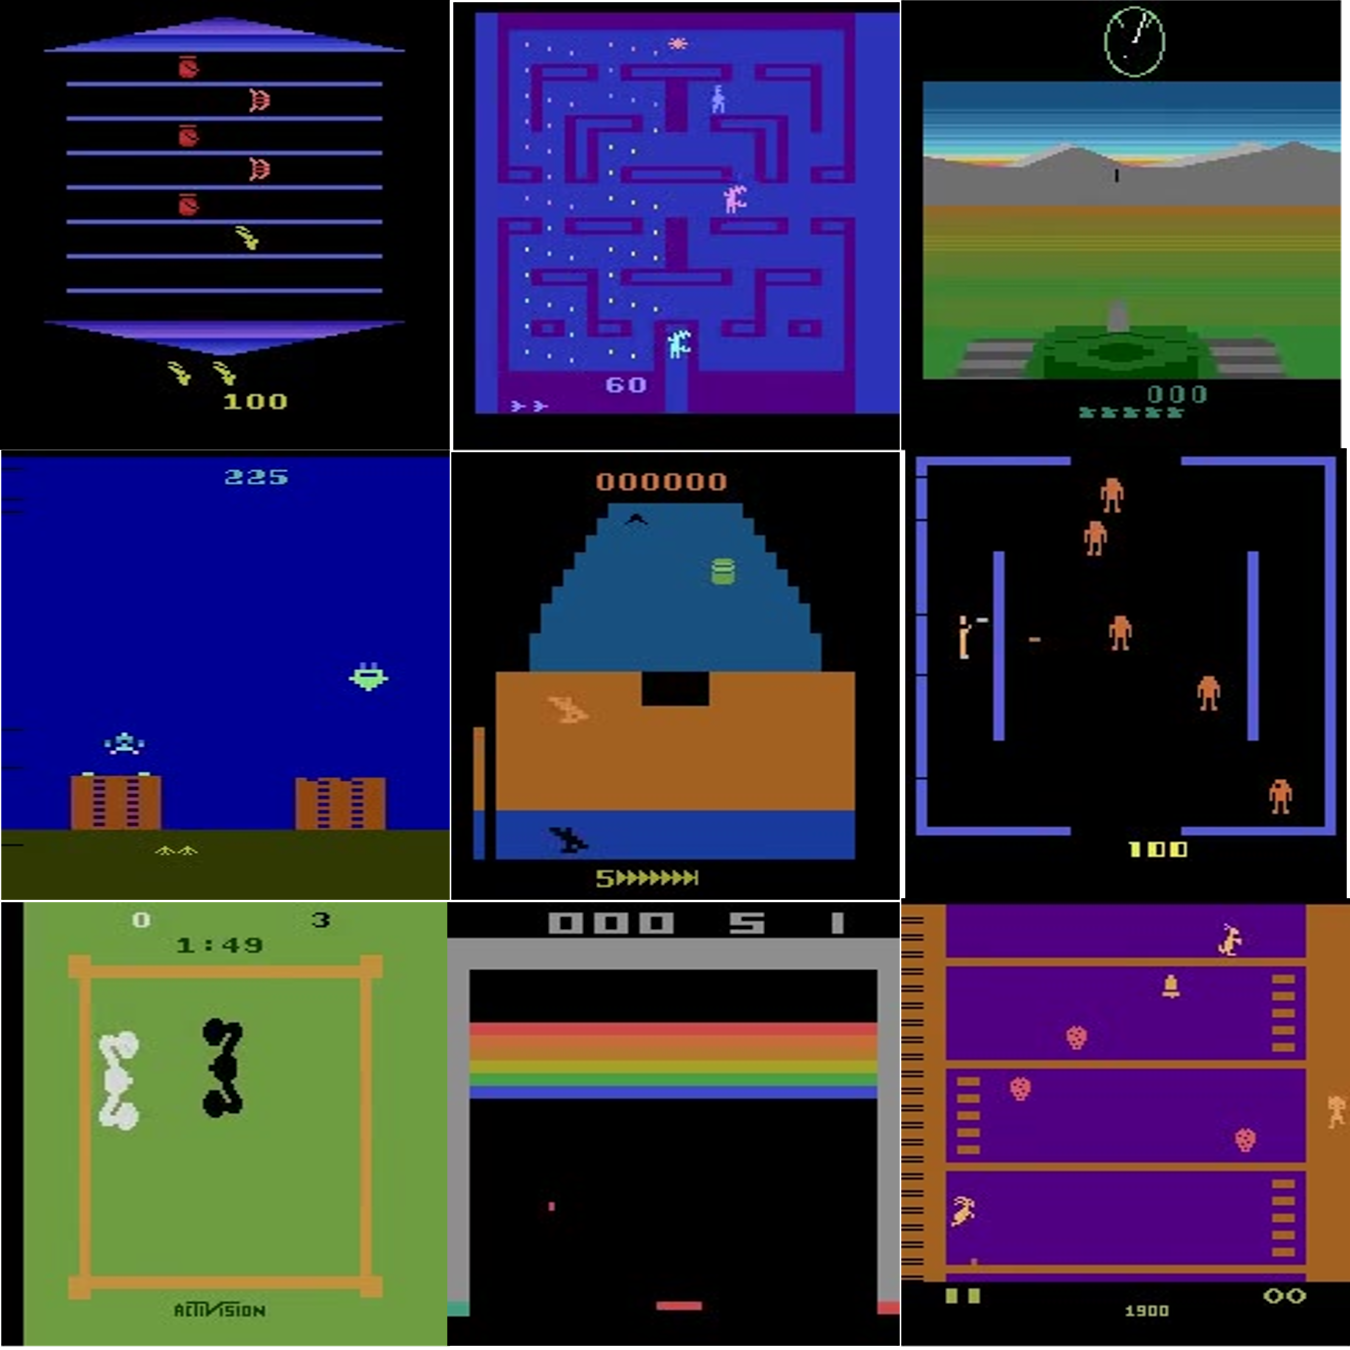
\includegraphics[scale=0.15]{img/openai_gym_environment.png}
\caption{Different kind of Atari Games environment available in OpenAi-Gym}
\end{figure}
\clearpage

\hfill \\
This framework makes it really easy to implement RNN in environment well formated. Fortunatly, the community have already build a OpenAI-Gym environment for the DonkeySimulator: Gym-Donkeycar


\subsubsection*{Gym DonkeyCar}

Thanks to Tawn KRAMER\cite{GymDonkey}, we have a pre-made environment following the OpenAI-Gym methodology. It basically runs a TCP connection with the simulator and transform the data received into Python formated data. This way, we don't have to create the TCP client by ourself\footnote{Although we tried doing it cf. appendix \ref{TCPClient}}

 The same component are implemented as follow:\\

\texttt{Observation} is a \texttt{np.array} with a shape of (120, 160, 3).\footnote{Basicaly it's the RGB representation of a 120x160px image}\\

\texttt{Done} is a \texttt{boolean} set to \texttt{True} when the car hit an obstacle (\texttt{hit != "none"}) or when it's too far from the center of the lane.\\

\texttt{Reward} is an \texttt{array} containing \texttt{Done}, the \textbf{speed}\footnote{Between max=1 and min=-2} of the vehicule and the \textbf{Cross Track error} (cte)\footnote{How far the car is from the center of the lane}\\

\texttt{Info} is an \texttt{array} containing the \textbf{cte}, the \textbf{position} (x,y,z), the \textbf{speed} (positive forward, negative backward) and if the car has it an obstacle: \textbf{hit}  (equal to "none" if all good)\cite{DonkeySim}

With all these information, we can feed the network with the \texttt{Observation} and make it output a steering angle and a throtle value.\\

It's quite funny to watch the IA train, because it's basically running all over the place at first, but then it start going further and further on the track. Sometimes you can have a big gain from a step to an other, or the AI can even regress ! But in the end, after a few hours of training, the AI is finaly able to drive through the whole track !

\begin{figure}[H]
\centering
\begin{minipage}{6cm}
\centering
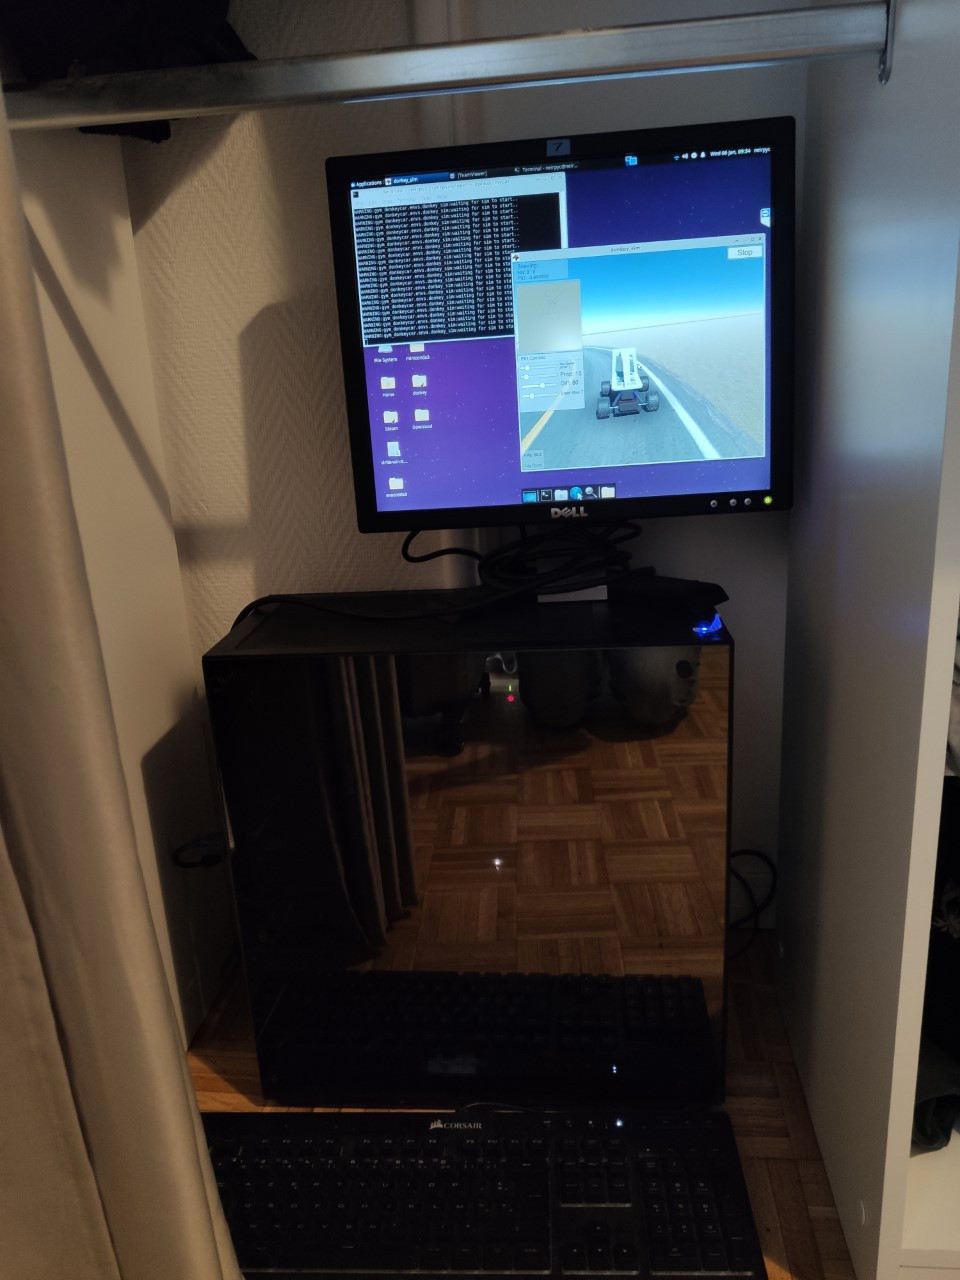
\includegraphics[scale=0.13]{img/linux.jpeg}
\caption{The Linux server we used for our training : \makebox{Xeon X5650 (6 cores 12 threads)}  8Go DDR3 - Nvidia GTX 970 4Go}
\end{minipage}
\hspace{2cm}
\begin{minipage}{6cm}
\centering
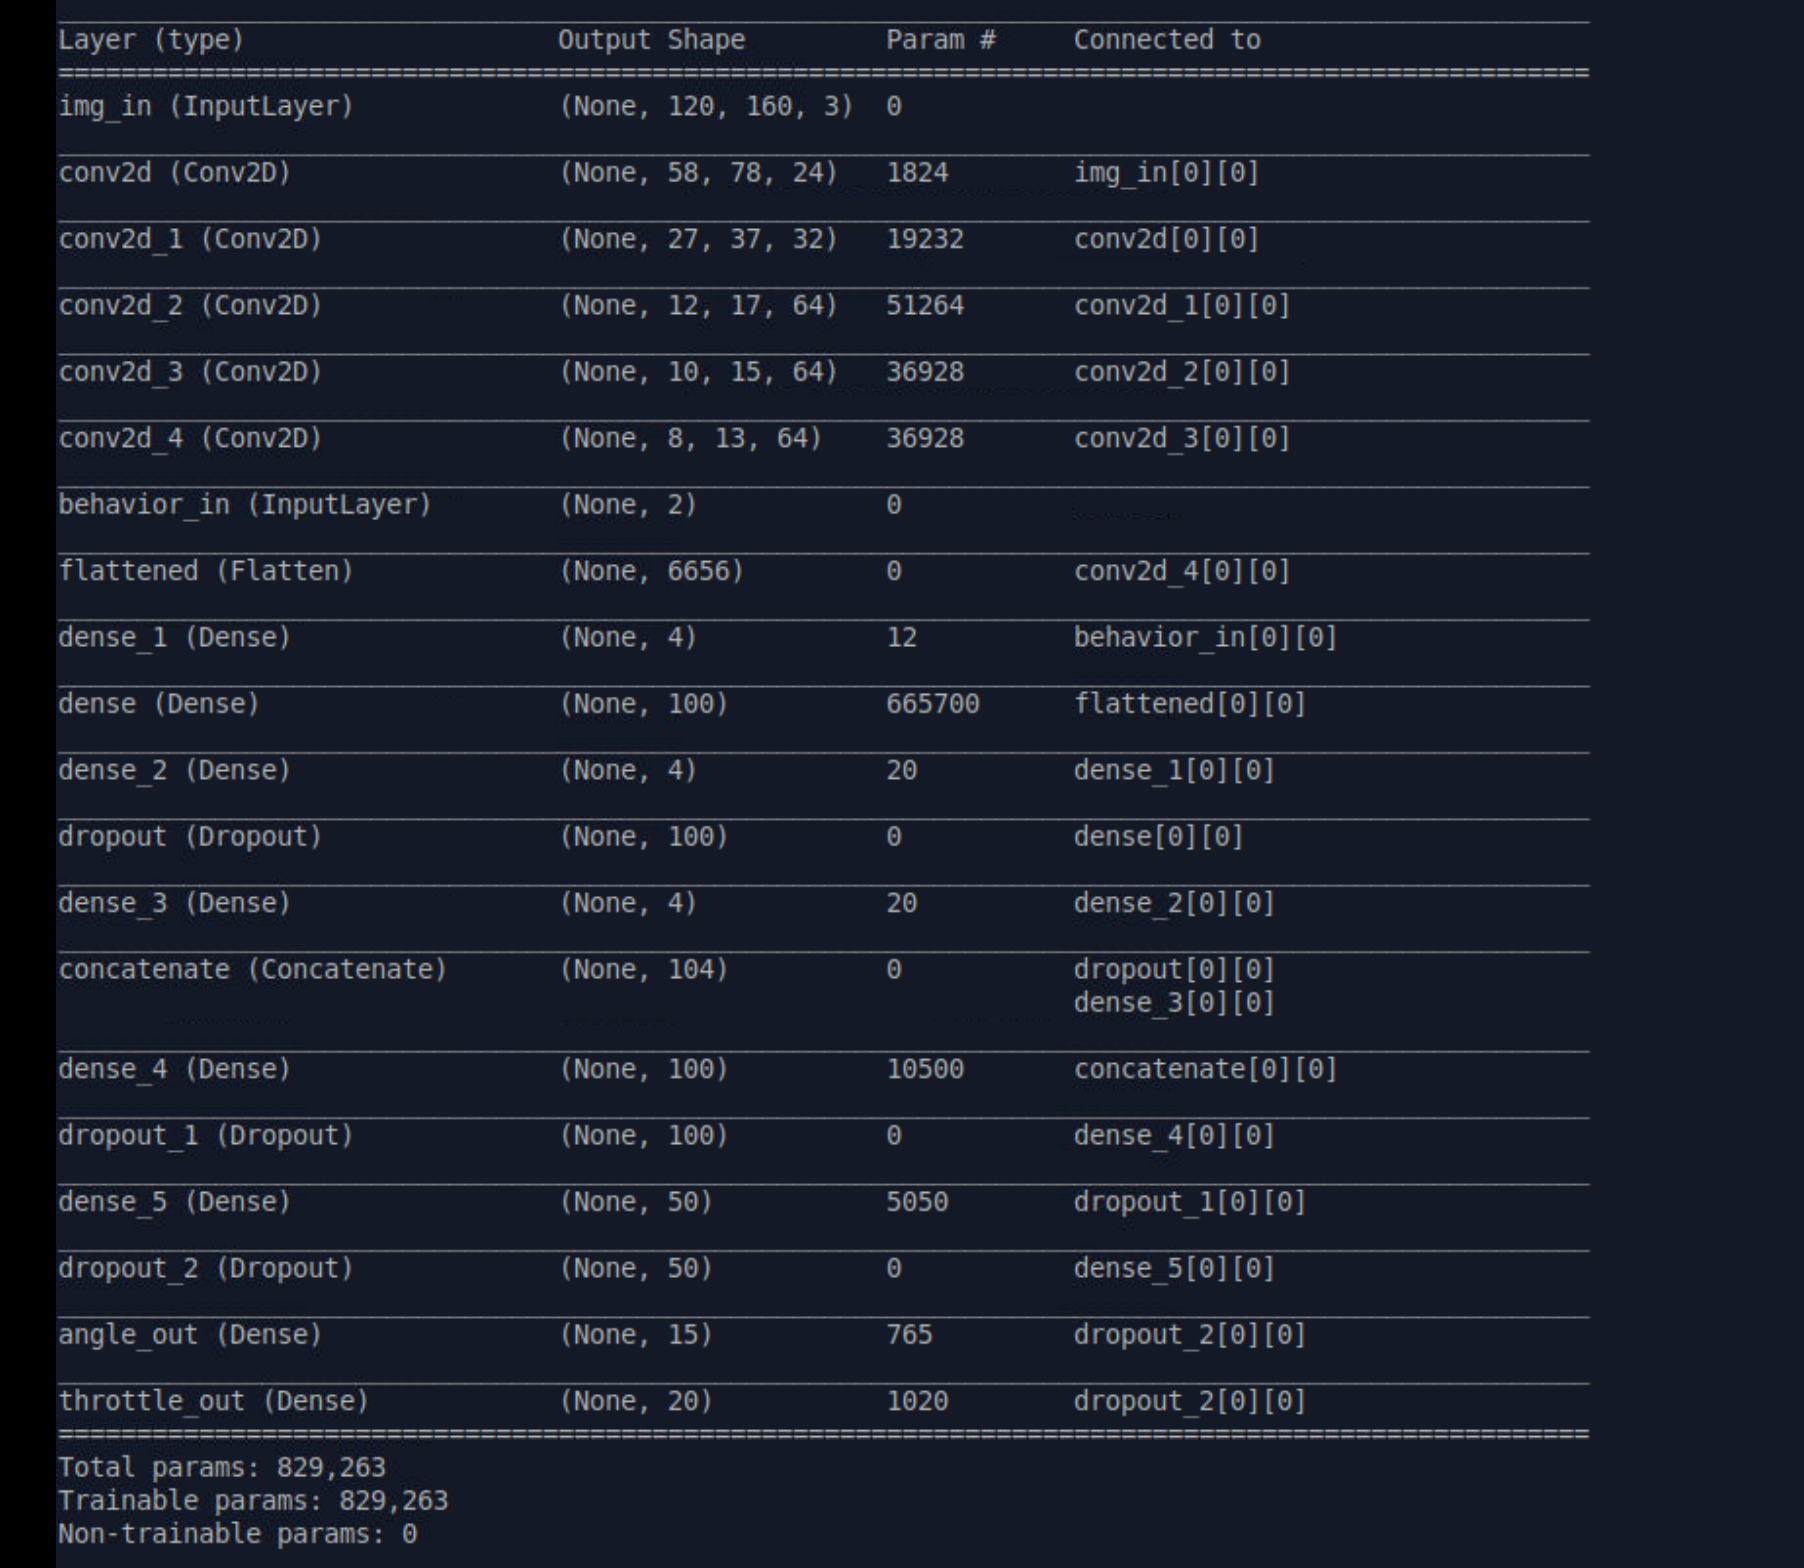
\includegraphics[scale=0.13]{img/keras.png}
\caption{example model run}
\end{minipage}
\end{figure}

\clearpage
\subsection{Benchmarks}

Using the DonkeySimulator, we ran 4 differents algorithms (unfortunatly we were not able to compute neither the imu nor the behaviour model), all in the same conditions, in order to compare their performances :\\
We used 9143 training images that we split in 7314 training images and 1829 validation images. 57 steps have been run each epoch.


\begin{figure}[!h]
\begin{minipage}{8cm}
\centering
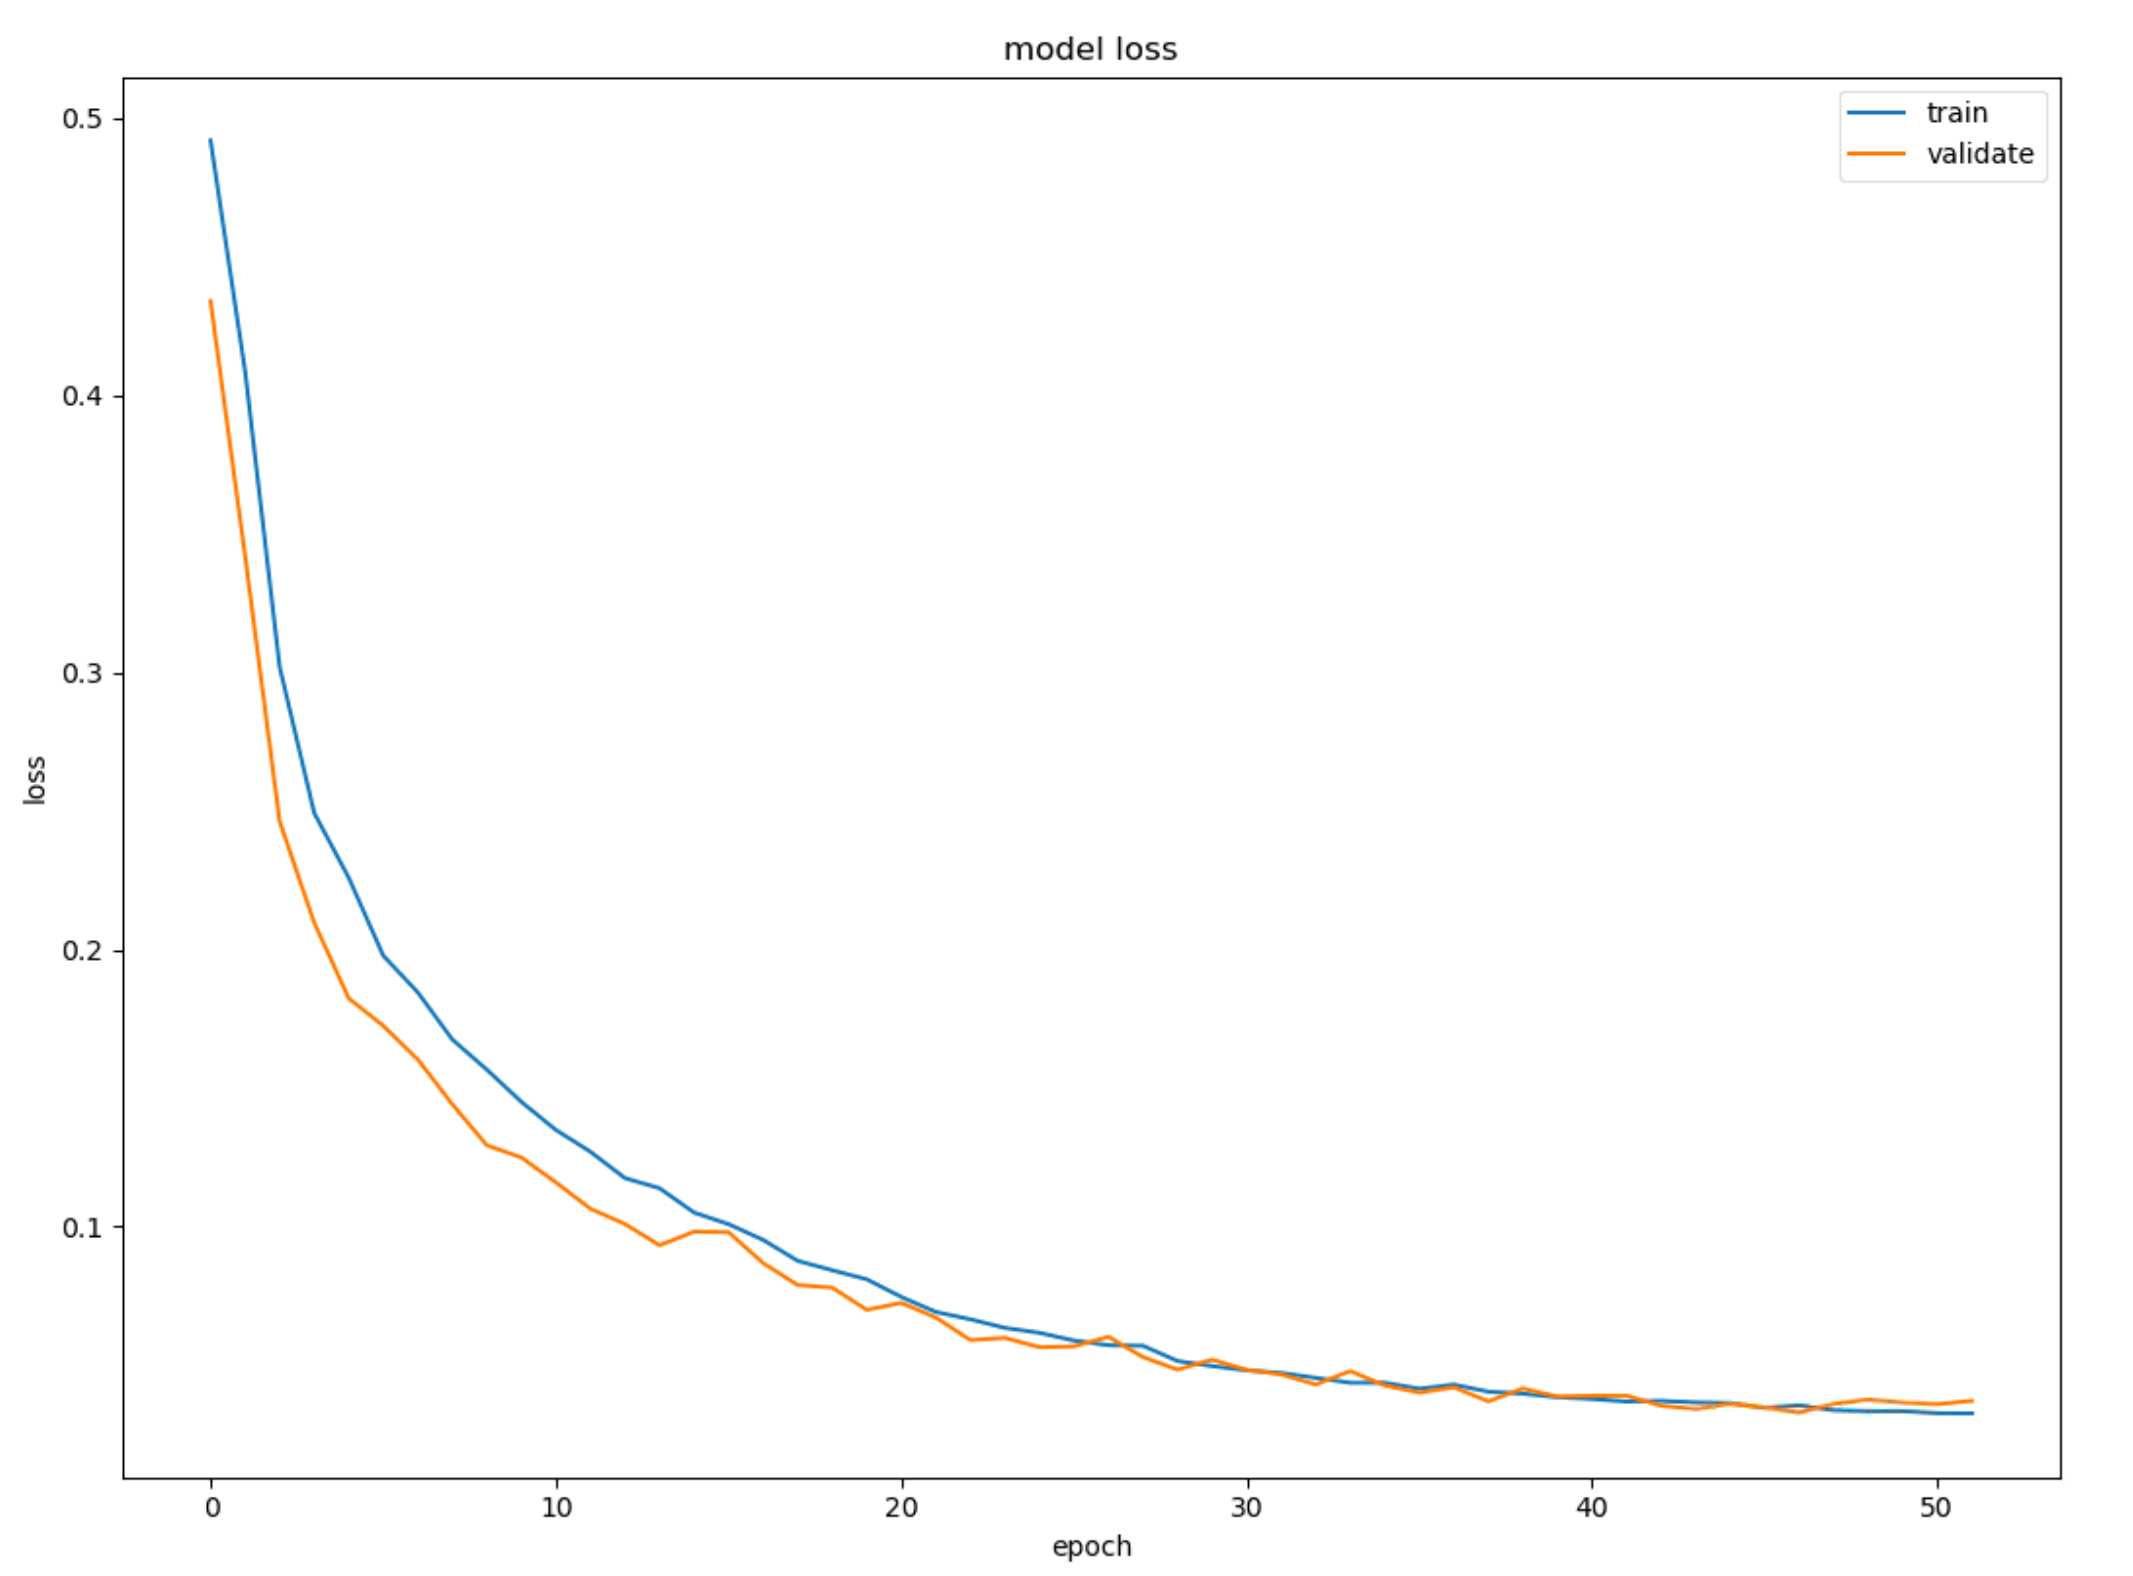
\includegraphics[width=8cm]{img/model_bench/linear.png}
\caption{Linear model loss}
\label{Linear model loss}
\end{minipage}
\hspace*{1cm}
\begin{minipage}{8cm}
\centering
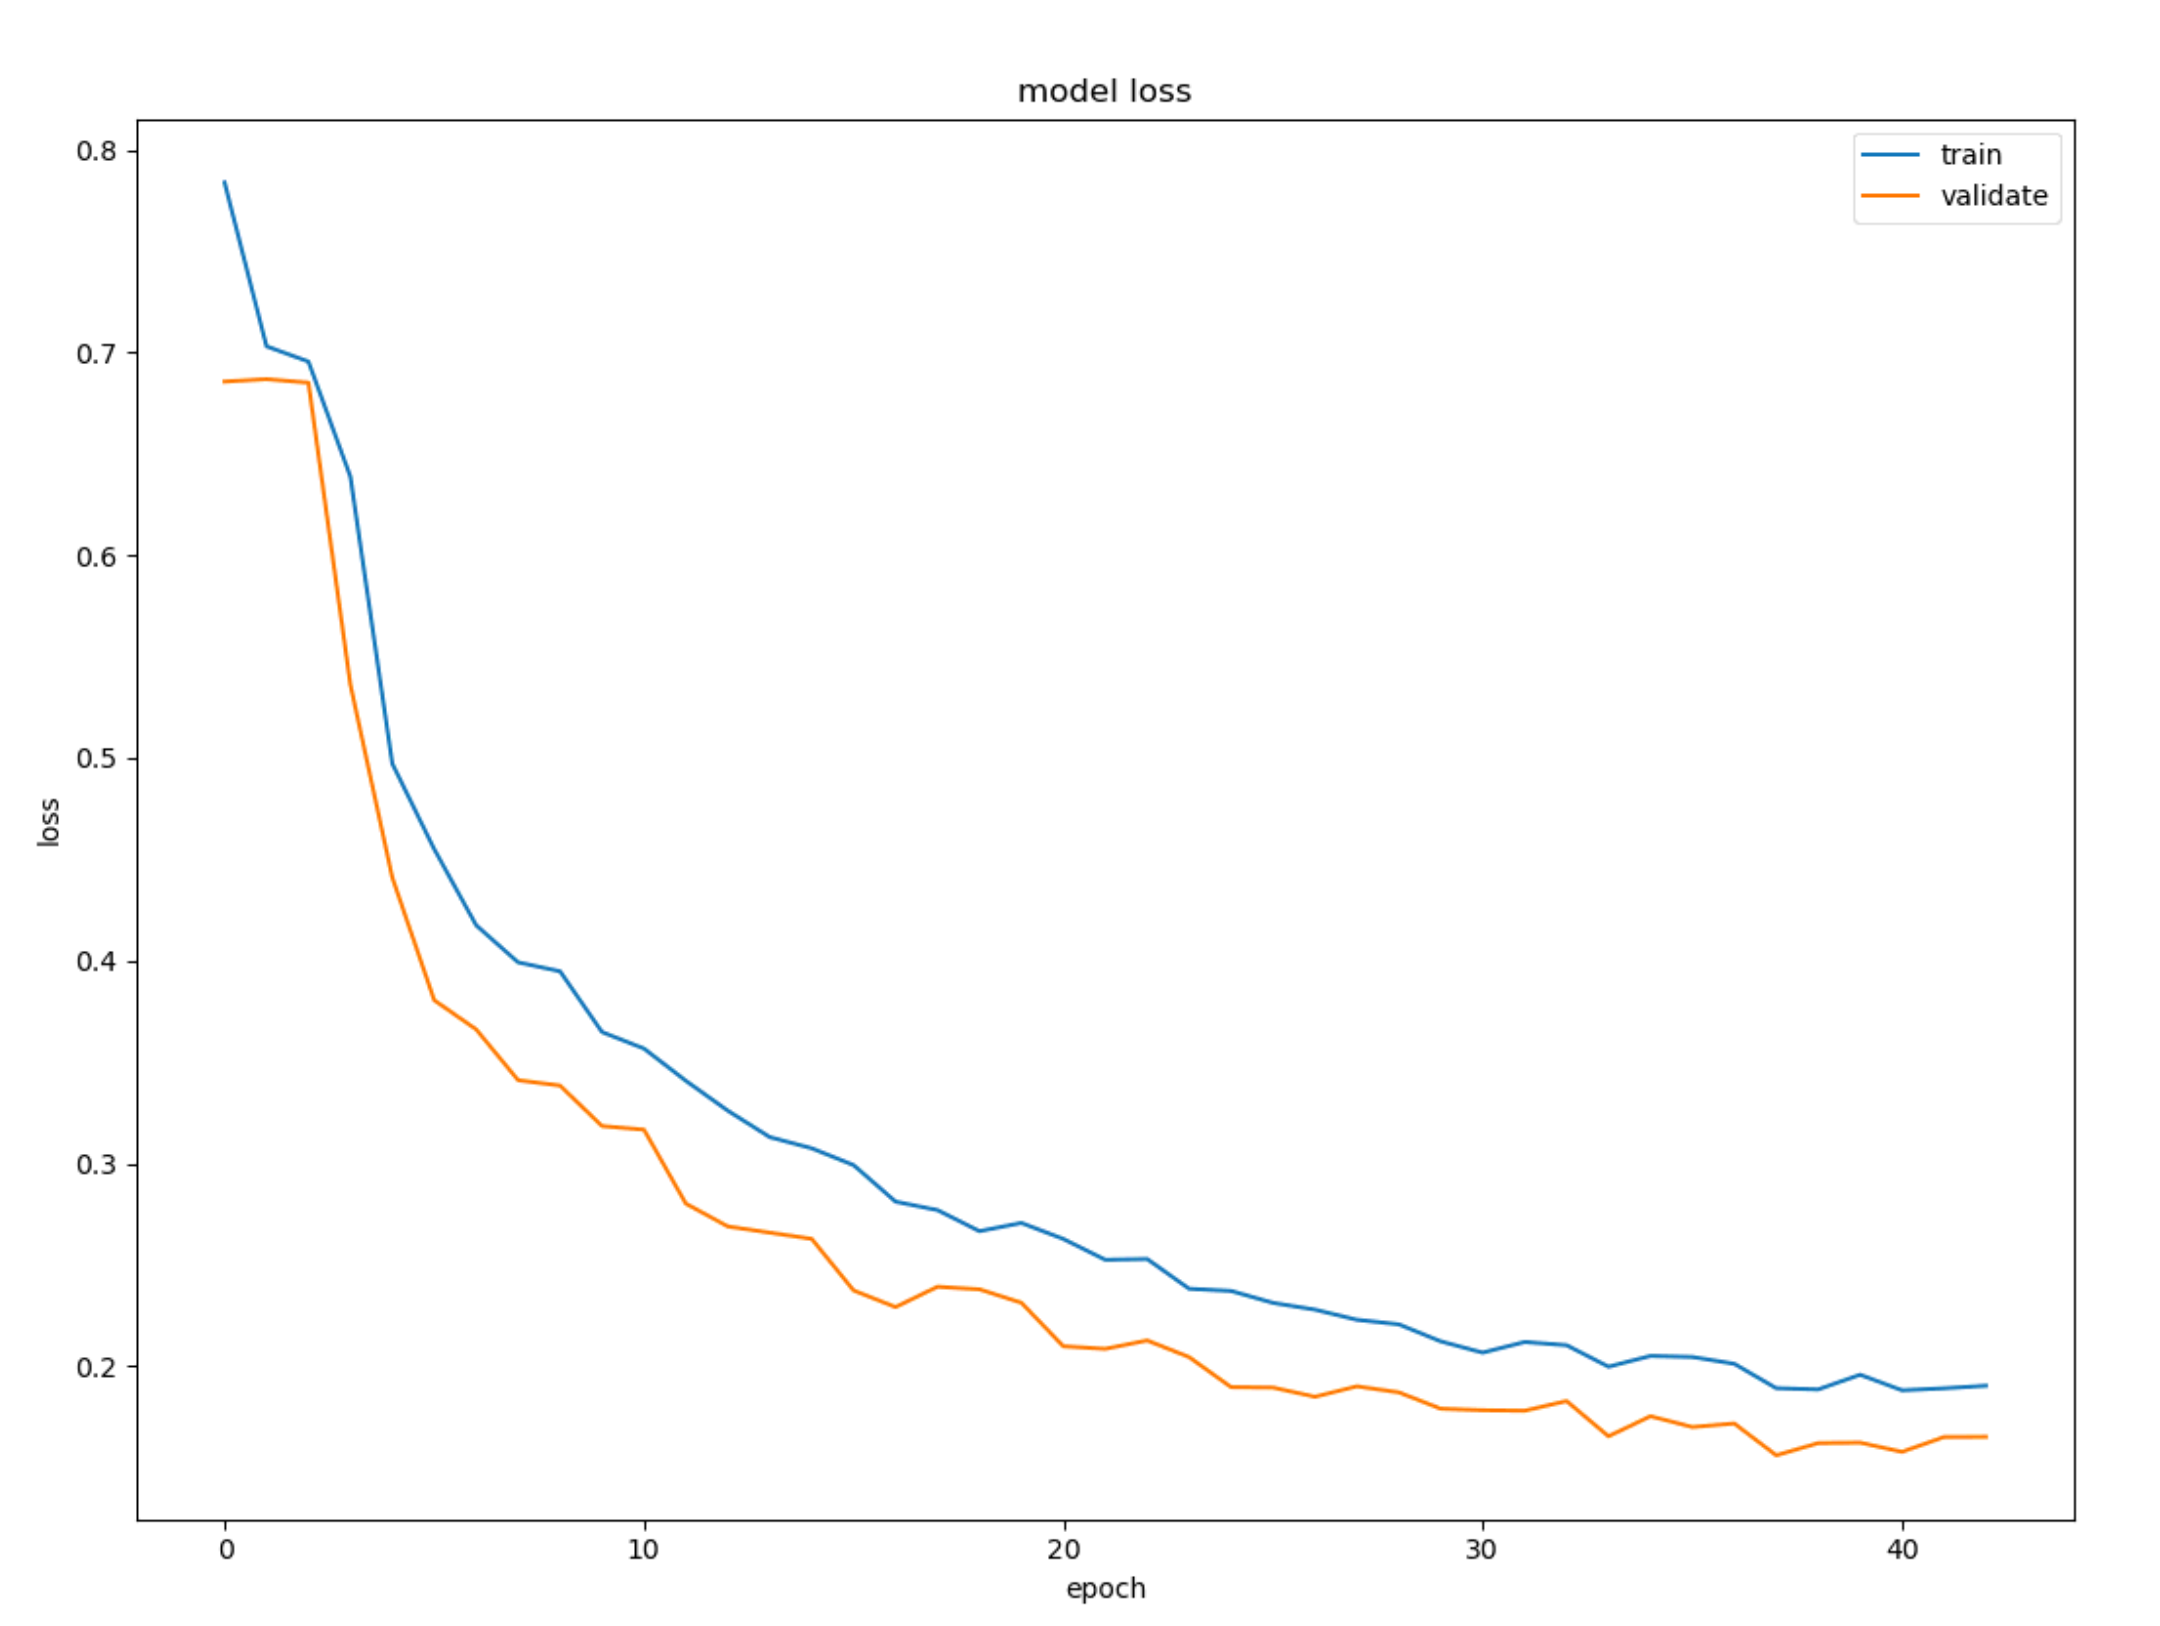
\includegraphics[width=8cm]{img/model_bench/latent.png}
\caption{Latent model loss}
\label{Latent model loss}
\end{minipage}
\end{figure}

\begin{figure}[!h]
\begin{minipage}{8cm}
\centering
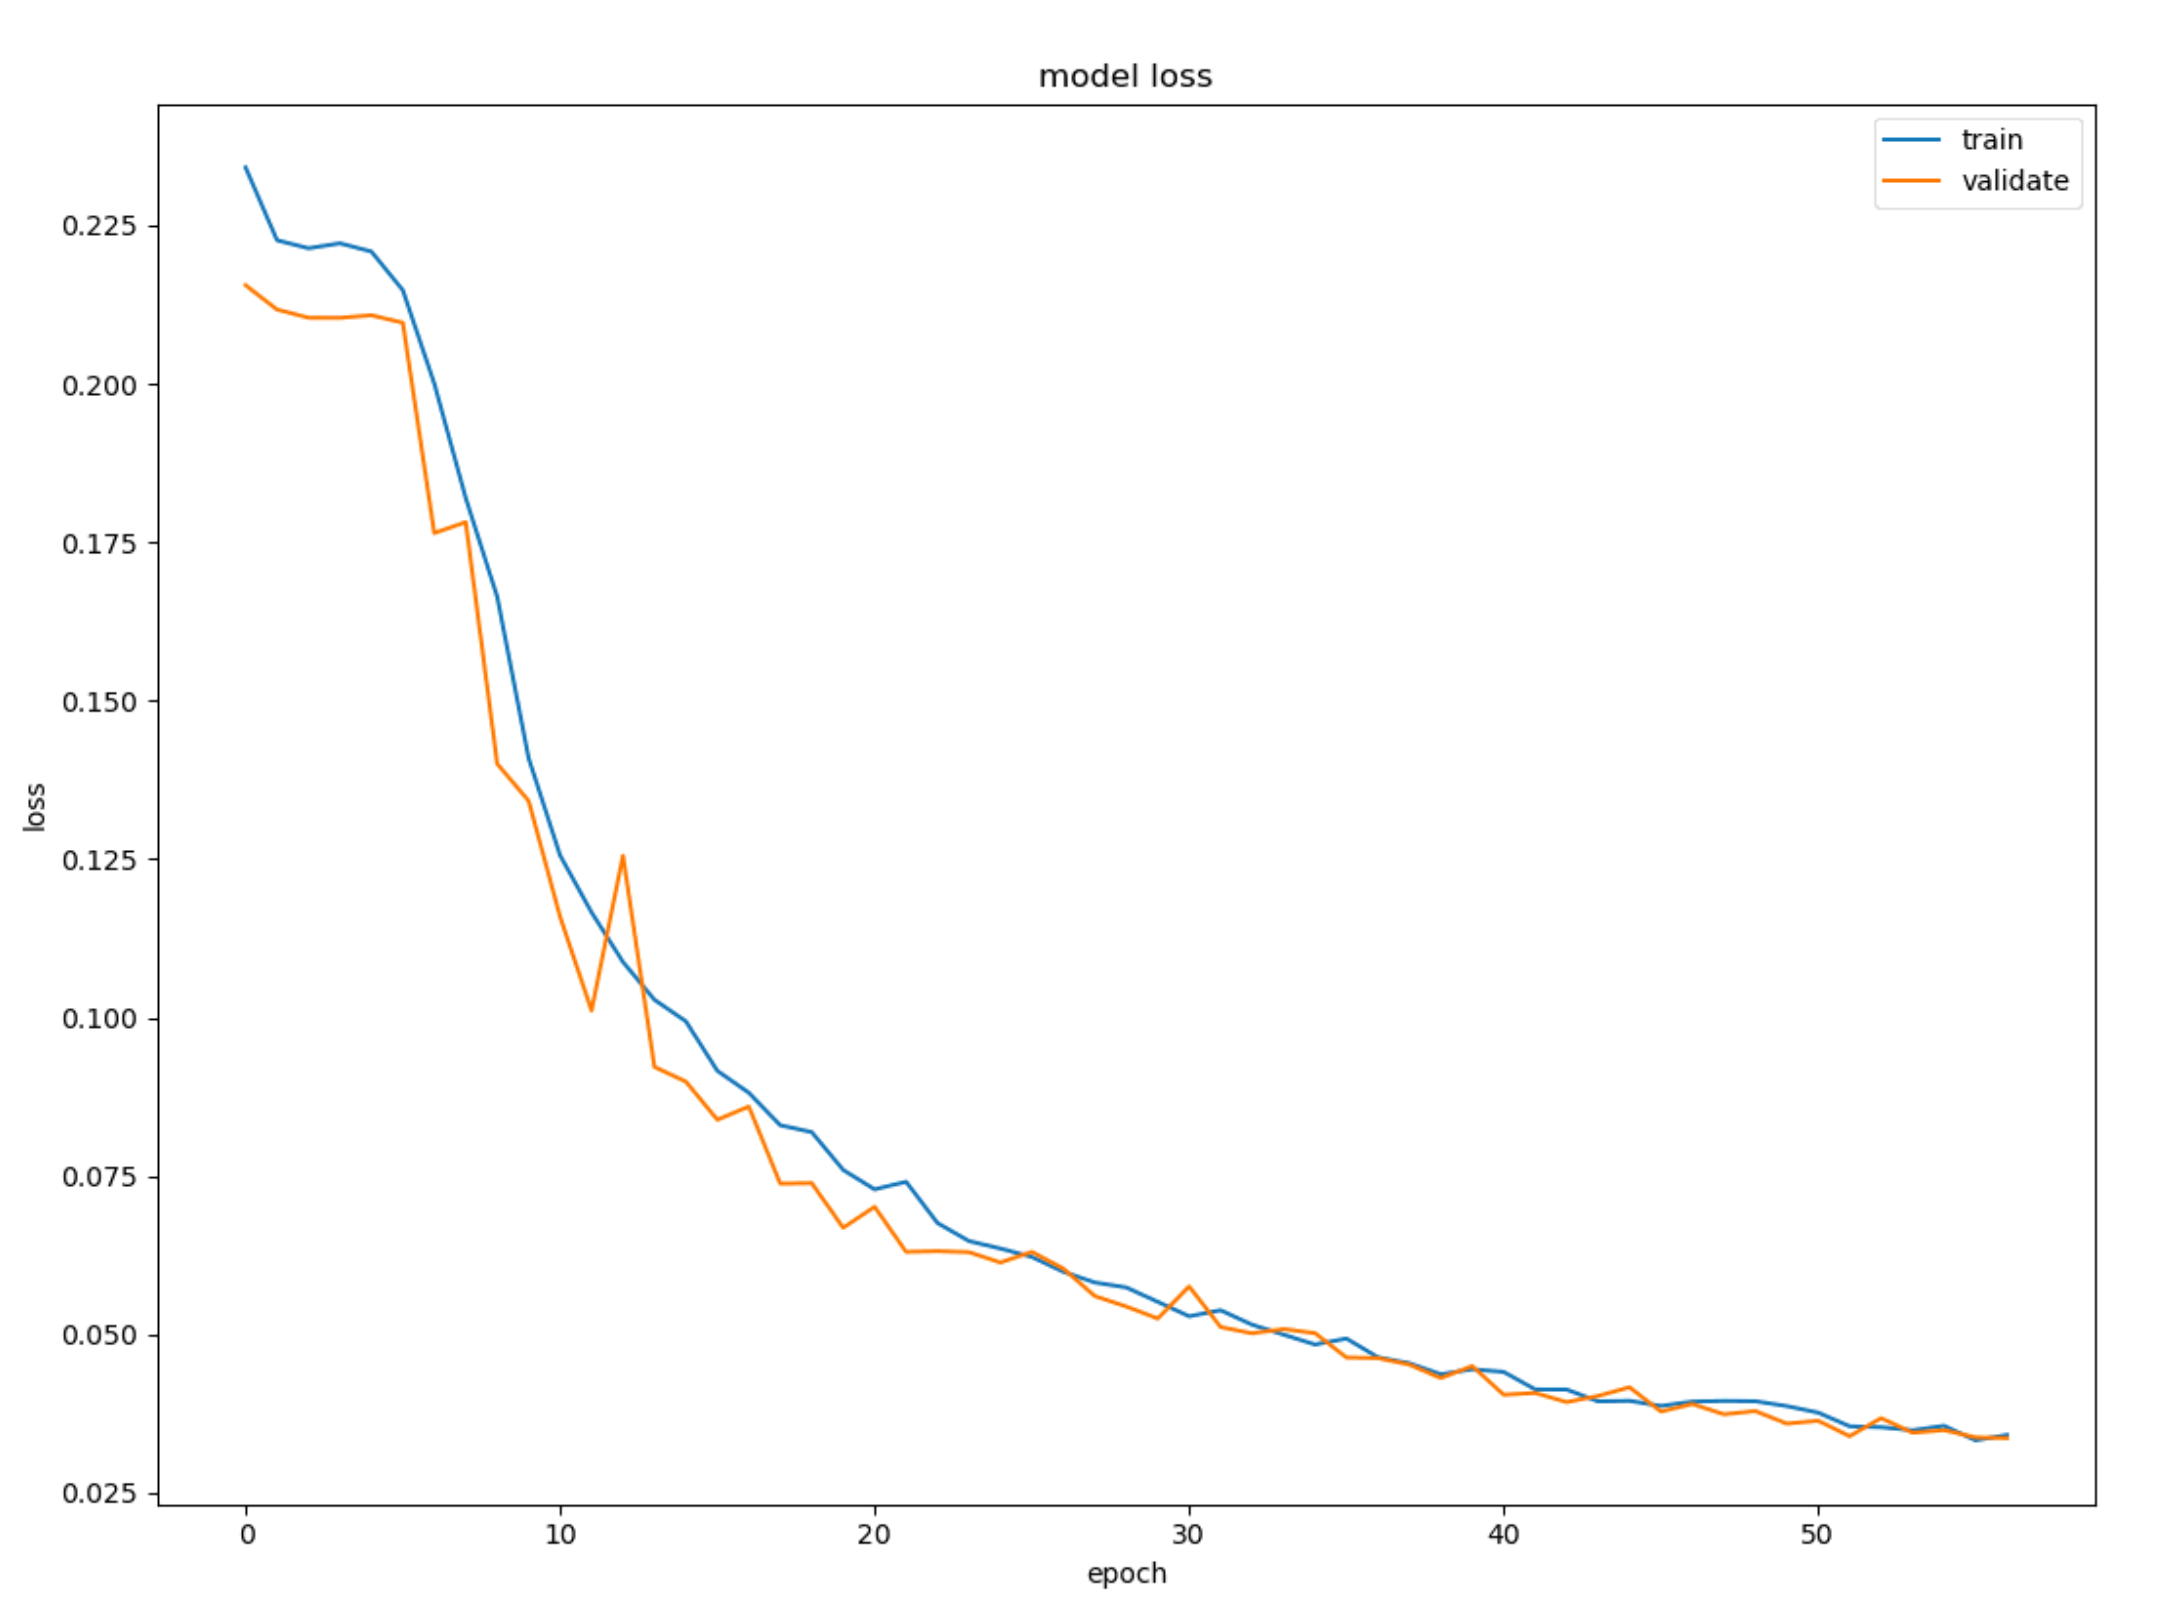
\includegraphics[width=8cm]{img/model_bench/rnn.png}
\caption{RNN model loss}
\label{RNN model loss}
\end{minipage}
\hspace*{1cm}
\begin{minipage}{8cm}
\centering
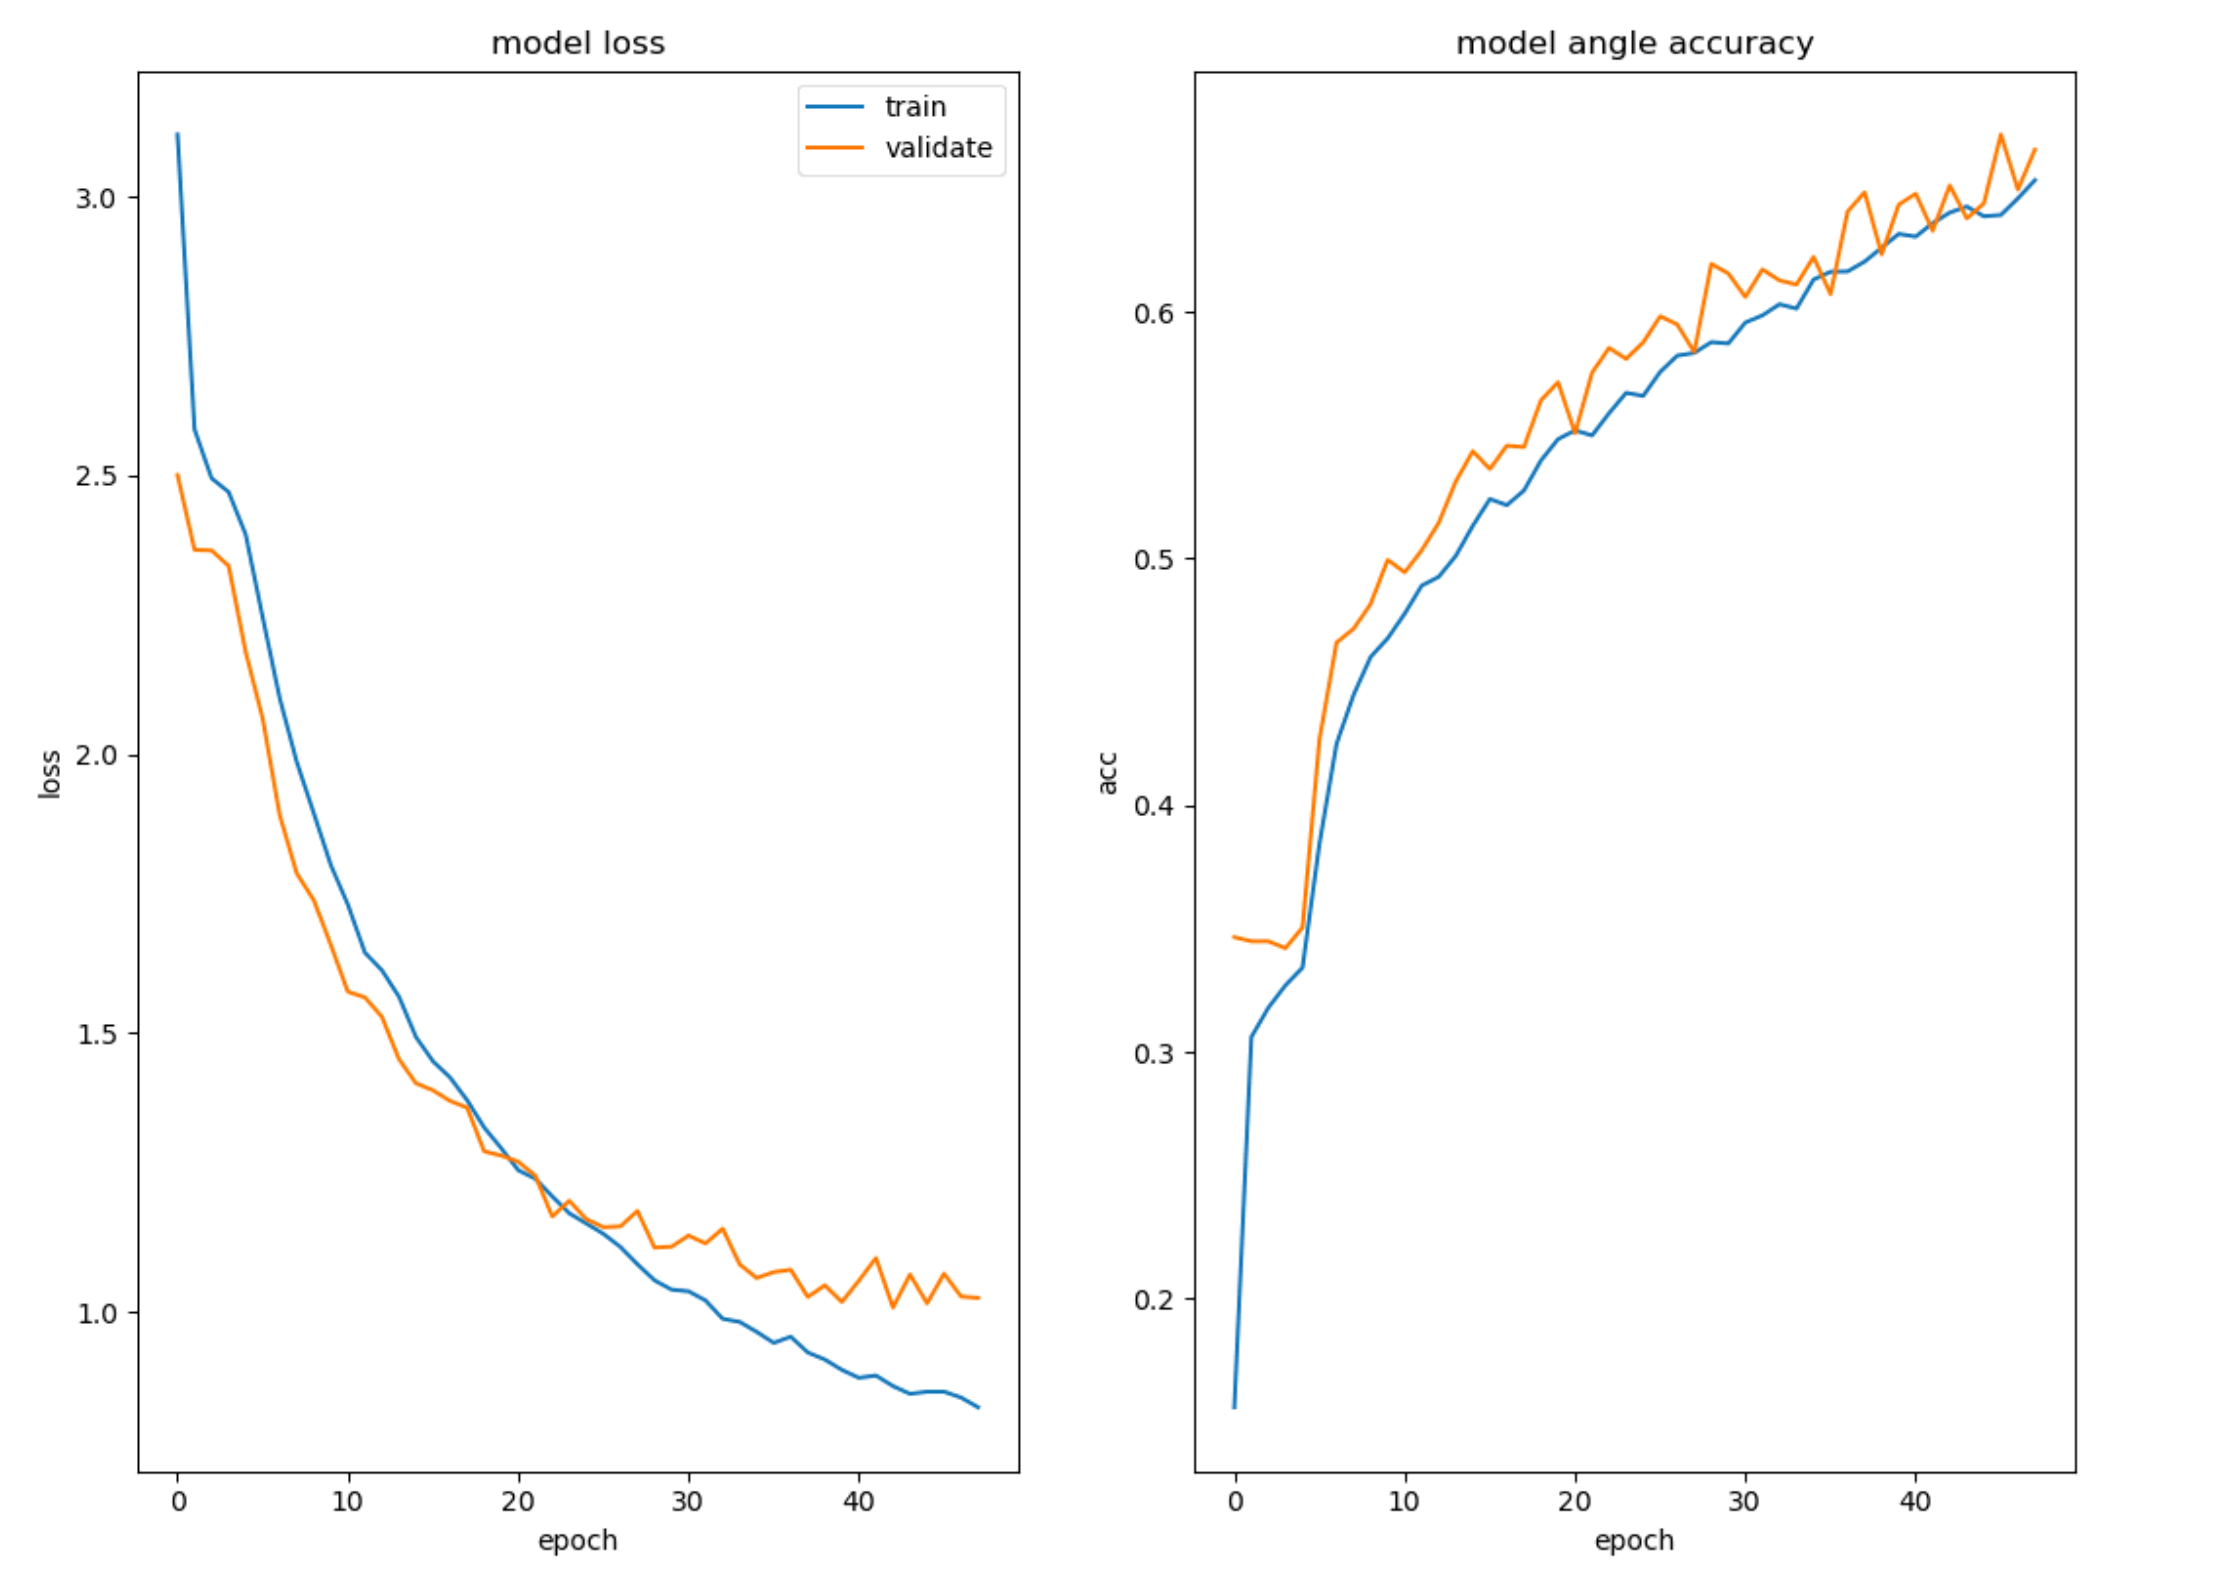
\includegraphics[width=8cm]{img/model_bench/categorical.png}
\caption{Categorical model loss and model angle loss}
\label{Categorical model loss}
\end{minipage}
\end{figure}

We can see that the \textbf{Linear} (Fig. \ref{Linear model loss}) and \textbf{RNN} (Fig.  \ref{RNN model loss}) model we used fit pretty well the data, but in the other hand, the \textbf{latent} (Fig. \ref{Latent model loss}) model tend to underfit the data while the \textbf{Categorical} (Fig. \ref{Categorical model loss}) model seems to overfit it.\footnote{The categorical model has 2 plot, one for the model angle accuracy and one for the model itself, that's because it's first trained on angle only and then on both throttle and angle.} \\

Even though the linear model look pretty well suited for the task, in practice, we found that it tends to oscilate way more than the RNN model. A solution to this kind of problem would be to implement a PID controler to smooth the driving, but this will be a way of improvement for the final model. 
\clearpage
\begin{figure}[H]
\centering
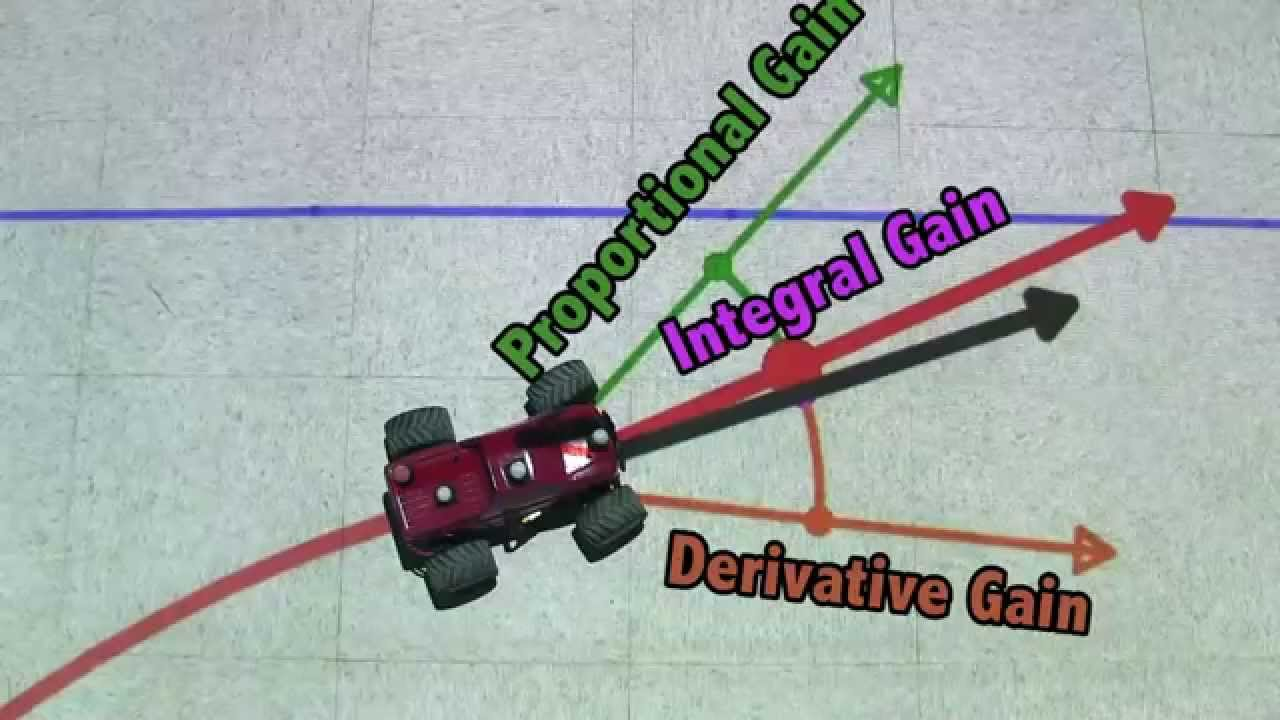
\includegraphics[scale=0.3]{img/PID.jpeg}
\caption{A PID Controler}
\end{figure}









\clearpage

